\section{Methodology}
%What was done.
As indicated by the posed research queries in Section \ref{sec_res_q},
this project consisted of two distinct development tasks:

\begin{itemize}
\item Implementation of a SLAM solution on a Thymio II robot.
\item Parallelisation of the existing Thymio simulator.
\end{itemize}

Due to the loose coupling of the simulator and the SLAM implementation, each of
the development tasks could be conducted in parallel by individual project
members.

Overall, this resulted in a project consisting of three components working
together:
\begin{itemize}
    \item The robot control code, implementing SLAM and other behaviours
        on top of it.
    \item A simulator based on Aseba Playground, but reduced in size and
        resource consumption to allow faster or parallel execution.
    \item The Thymio II robotic platform to be controlled.
\end{itemize}
By maintaining a common and known interface shared by the Thymio II and the
simulator, the SLAM software could be tested and executed against the simulator
and the Thymio itself identically, meaning that no additional support, or glue,
code would be required that may distort results between what are observed on
the simulator and in real life. In essence, the control code cannot ever
identify the difference between the two.

The methodology and development techniques of each deliverable is detailed
below.

\subsection{SLAM Solution}\label{meth_slam}
%What was implemented on the robot and limitations of the platform.
As has been previously detailed, SLAM solutions consists of three main
operations:
\begin{itemize}
    \item Robotic movement
    \item Obstacle observation
    \item Map update
\end{itemize}
The three SLAM steps provided a simple and intuitive manner to divide the
implementation of an algorithmic solution of the SLAM problem.

\subsubsection{Robotic Movement}
The navigational portion of a SLAM solution requires a robot to not only move
through an area, but to also keep an approximate record of how each movement
has altered it's position in the environment.

There are two main approaches to allow a robot to estimate is position
without external aid; odometry and dead-reckoning.

Odometry is considered the preferable option for estimated localisation, as
the motion sensors required for implementing the feature can be extremely
reliable, resulting is very accurate estimations.
The alternative solution to onboard localisation estimation is via
dead-reckoning - where location is estimated based upon the speed that the
robot was travelling.
The basic dead-reckoning calculation is identical to the kinematic
distance formula:

\[ D = V \times T \]

Where the distance travelled \(D\) is equal to the product of velocity of
movement \(V\) and the time spent travelling \(T\).

As the Thymio II's wheels were not equipped with any form of rotary encoders,
native odometery was not possible, and thus dead-reckoning had to be used for
localisation estimation.
Though Thymio systems have been utilised as testing platforms in multiple
studies, including SLAM solutions that utilise dead-reckoning, the Thymio II
system does not include dead-reckoning `out-of-the-box' and thus a bespoke
implementation had to be developed.
Investigation into previous implementations of dead-reckoning on a Thymio
system revealed little usable or adaptable software that could be utilised for
this project.
The only code relating to Thymio II estimated location was found in a
navigation driver plug-in for the Robot Operating System (ROS) - an open-source
middle-ware for robot control.
As the Thymio II used in this study was not utilising ROS as system driver,
the navigation plug-in could not be implemented directly - but still provided
significant insight into how the bespoke dead-reckoning could be implemented.

The ROS Thymio II navigation driver indicated that a unmodified Thymio II
robot had a speed coefficient - or hypothetical speed of 2.93.
Ad hoc experimentation using the Aseba simulator revealed that ROS navigation
module's estimated speed coefficient was accurate, but this value was not
representative of the real-world robot.
The Thymio II robot utilises an integrated battery to power itself, and
during operation the internal voltage of the battery is drained.
Unfortunately, due to the lack of power regulation, as the voltage of the
internal battery dropped, so to did the speed of the robots wheels.
The inconsistent speed at which the wheels operated meant that the
constant speed coefficient extracted from the ROS package could not be used to
accurately determine the location of the robot - as the longer that the robot
was mobile, the slower its wheels would operate, resulting in more inaccurate
predictions as time moved on.

A second issue regarding robot's mobility was also discovered during the
experimentation process - the Thymio II's inability to travel in a straight
line.  
The Thymio robotic platform's movement operations are controlled by issuing
commands to change the speed and direction of each wheel individually - by
setting both wheels to the same speed and direction the robot should move in a
straight line.
Experimentation revealed that left wheel of the Thymio II utilised in this
project was unable to match the same speed as the right wheel - causing the
robot to curve leftwards when attempting to move directly forwards.
The cause for this issue was unapparent, but a number of possible reasons were
considered:

\begin{itemize}
\item Friction between the wheel and robot chassis.
\item Unbalanced power regulation.
\item Poor production tolerances.
\end{itemize}

A theorised solution was to limit the speed of the rightmost wheel to
percentage of the left.
While theoretically sound, the proposed solution proved futile, as the speed of
the robot's wheels were coupled non-linearly to the voltage of the internal
battery - resulting in the robot once again curving as the maximum speed of
the robot slowed.

While it was not possible to implement a reliable dead-reckoning
system on the physical robot, there was still potential for the estimated
localisation to function correctly within the perfect conditions of the
simulated environment, and thus development moved to the next stage of the
SLAM problem.

\subsubsection{Obstacle Observation}
To be a valid SLAM solution, a robotic agent is required to observe the
environment around its self in order to identify landmarks or features which
can be utilised by the robot to localise its self in the global environment.

As outlined in Section \ref{tools_robot}, the Thymio II robot featured five
forward facing infrared sensors, with a documented effective range of \~{}10cm.
Preliminary experimentation was conducted to verify that the Thymio's
documentation was accurate.
Investigation revealed that the operational tolerances of the Thymio's sensors
was not consistent, with the majority of the infrared sensors only able to
consistently detect objects within a range of \~{}6-8cm.
The extremely limited range of the sensors made the task of object detection
excessively complex, as a robot would not be able to observe environmental
features without moving within close proximity of a map obstacle.
The short range of the sensors also limited the execution of the third SLAM
solution step; the updating of the agent's map.

\subsubsection{Map Update}
The final step of this projects proposed SLAM solution was to update the
robotic agent's approximated map of the environment.
The process of updating a map consisted of two steps; determining if the
obstacle currently being observed was already recorded in the map, and in cases
where the obstacle has not been recorded, adding the new features to the map -
using previously identified landmarks as references. 
As previously stated, the Thymio II's extremely limited sensor capabilities
made the implementation of the map updating task practically impossible.

In order to correctly add new features to the internal map, a robotic agent
must first determine where the obstacle exists in a global context.
This is achieved by the robot utilising its sensors to locate the position
and distance of a previously observed map feature, and calculating the new
feature's distance from this known location.
The robot can then utilise the result of this calculation to add the estimated
location of the new feature to the approximated map.

Due to the Thymio II's sensors possessing a maximum effective range of around
6cm, the robot would not be able to accurately determine the location of an
obstacle that was placed more \~{}12cm away from any other environment feature.

An environment containing objects dispersed no more the 12cm away from one
other would be extremely impractical to testing a Thymio II SLAM solution:
\begin{itemize}
\item The close proximity of the obstacles would complex the process of
differentiating new features from previously observed features.
\item The Thymio II's dimensions measure 11cm by 11.2cm, making navigation of
\~{}12cm paths extremely difficult, to borderline impossible - due to the
unreliability of the Thymio's wheel motors.
\end{itemize}

As was the case of dead-reckoning, neither obstacle observation, or map
updating could be implemented on the physical robot due to constraints of the
native hardware.
It is feasible that a simulated implementation of the obstacle observation and
map updating could be produced, however alterations would first have
to be made to the simulator in order to increase the range of the artificial
Thymio II's sensors - which originally matched the documented range of the
real-world counterpart.

\subsection{Simulator}
As stated, the aim of the simulator modifications was to reduce the resource
consumption and increase the speed of the simulator, to allow more strategies
or behaviours to be tested before execution on the physical robot platform.

To this end, the source code for the Aseba Playground was inspected to
understand its structure, makeup, bottlenecks, and pliability to the project
aims. After some time analysing the system and benchmarking its performance,
it was determined that the large Qt GUI application was unsuitable to be pared
down. Instead, it would be deconstructed into its component parts, and a new
simulator and set of tools built in its place.

Although the new simulator would differ internally, it was important that the
implementation would replicate still the same outward interfaces of the
playground, but also that of the robot. In doing so, the simulator would be a
drop in replacement for these other components, meaning that the SLAM control
code would not need different modes or interfaces to talk to the robot than it
did to the simulator. This would be advantageous if the project were to advance
down other methods of control, such as evaluating behaviours programmatically,
where the measured outcomes would be based on the result of the simulation, as
though to the control code it was actually functioning in the real world.

With this in mind, the each of the components identified previously were
considered for their necessity in a new, minified simulator. Of these that were
considered vital, their size and complexity was also evaluated, and where
possible, replaced with a smaller implementation expressing the same interface.
The total architecture with the Playground is shown below.
\begin{figure}[!h]
    \centering
    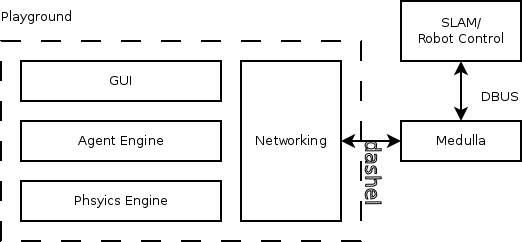
\includegraphics[width=\textwidth]{playground.png}
    \caption{Architecture of the Aseba Playground simulator, and its relation
    to robot control code.}
\end{figure}

Ultimately, the following components were kept, in part, or by reimplementation:
\begin{itemize}
    \item Physics engine - kept in full
    \item Agent engine - only the Thymio II agent retained
    \item Networking components - reimplemented minimally, implementing the
        Medulla switch interface.
\end{itemize}
The GUI was excluded, as visual output was not required. Additionally, much of
the support code, such as that used to load image files for graphical world
representation was also dropped.

\begin{figure}[!h]
    \centering
    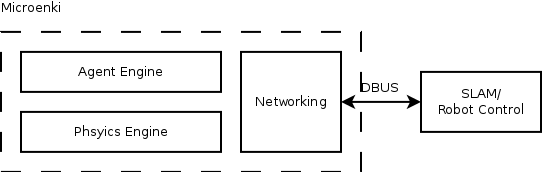
\includegraphics[width=\textwidth]{microenki.png}
    \caption{Architecture of the Microenki simulator, and its relation to
    robot control code.}
\end{figure}

The paring down of the simulator reduces the CPU resources consumed. As a result
more instances can be executed in parallel. Additionally, for a given segment of
time, less work needs to be done, allowing the code to execute more quickly. It
also reduces the memory consumption to host the simulator, again allowing more
instances to be hosted and executed simultaneously.

One of the options available to help accelerate the simulation would be to to
use a GPU. As simulations of physics can be highly numeric, such as the
calculation of gravity or accelerations on many instances of physics agents,
it was possible that GPU acceleration would be effective in reducing the time
repeating many simple calculations. If much of the CPU use in the simulator was
dominated by this type of code, then it would be effective.

In order to investigate this, the minimised but CPU-only simulator was
internally instrumented and its call graph and the time spent in various parts
of the code checked. If high amounts of time were spent in the physics loops,
then offloading these parts to a GPU would greatly speed up the simulation. In
fact, most of the time in physics-rich environments was spent in simple memory
management routines, adding, removing, and testing for objects in the arrays
used to store and track the objects. This lack of suitability to GPU
acceleration was a major blow to the intentions to speed up individual
instances, one of the main strategies considered alongside the parallelisation
of whole instances. These call graphs are presented as auxiliary information
in appendix B.

Once the implementation of a trimmed down simulation was complete, it was
measured for CPU consumption at the steady-state, for steady-state RAM
consumption, and simulation speed ratio - that is, how fast the simulation can
execute.

To measure the simulation speed ratio, the simulator is set to run for a fixed
span of simulated time - in this instance 10 seconds. The time taken to then
complete this time span is measured. 100 recordings of this regime are made,
and the first and last 10 measurements are discared to discount cache warming.
The remaining 80 measurements are then averaged, and the simulated timespan is
divided by the time taken to execute. The resulting number is the simultion
speed ratio, the number of simulated seconds per execution second.

For steady-state CPU and memory consumption, the simulation instead runs at a
fixed ratio (1:1, as a fair comparison with the Playground), and the CPU and
RAM consumption measured 10 times each over 10 executions. As before, the first
and last measurements in each are discarded, and the remaining central 80\%
are averaged.
